% Options for packages loaded elsewhere
\PassOptionsToPackage{unicode}{hyperref}
\PassOptionsToPackage{hyphens}{url}
%
\documentclass[
  11pt,
]{article}
\usepackage{amsmath,amssymb}
\usepackage{lmodern}
\usepackage{setspace}
\usepackage{ifxetex,ifluatex}
\ifnum 0\ifxetex 1\fi\ifluatex 1\fi=0 % if pdftex
  \usepackage[T1]{fontenc}
  \usepackage[utf8]{inputenc}
  \usepackage{textcomp} % provide euro and other symbols
\else % if luatex or xetex
  \usepackage{unicode-math}
  \defaultfontfeatures{Scale=MatchLowercase}
  \defaultfontfeatures[\rmfamily]{Ligatures=TeX,Scale=1}
\fi
% Use upquote if available, for straight quotes in verbatim environments
\IfFileExists{upquote.sty}{\usepackage{upquote}}{}
\IfFileExists{microtype.sty}{% use microtype if available
  \usepackage[]{microtype}
  \UseMicrotypeSet[protrusion]{basicmath} % disable protrusion for tt fonts
}{}
\usepackage{xcolor}
\IfFileExists{xurl.sty}{\usepackage{xurl}}{} % add URL line breaks if available
\IfFileExists{bookmark.sty}{\usepackage{bookmark}}{\usepackage{hyperref}}
\hypersetup{
  hidelinks,
  pdfcreator={LaTeX via pandoc}}
\urlstyle{same} % disable monospaced font for URLs
\usepackage[margin=1in]{geometry}
\usepackage{graphicx}
\makeatletter
\def\maxwidth{\ifdim\Gin@nat@width>\linewidth\linewidth\else\Gin@nat@width\fi}
\def\maxheight{\ifdim\Gin@nat@height>\textheight\textheight\else\Gin@nat@height\fi}
\makeatother
% Scale images if necessary, so that they will not overflow the page
% margins by default, and it is still possible to overwrite the defaults
% using explicit options in \includegraphics[width, height, ...]{}
\setkeys{Gin}{width=\maxwidth,height=\maxheight,keepaspectratio}
% Set default figure placement to htbp
\makeatletter
\def\fps@figure{htbp}
\makeatother
\setlength{\emergencystretch}{3em} % prevent overfull lines
\providecommand{\tightlist}{%
  \setlength{\itemsep}{0pt}\setlength{\parskip}{0pt}}
\setcounter{secnumdepth}{-\maxdimen} % remove section numbering
\ifluatex
  \usepackage{selnolig}  % disable illegal ligatures
\fi

\author{}
\date{\vspace{-2.5em}}

\begin{document}

\setstretch{1.25}
\clearpage

\hypertarget{materiais-e-muxe9todos}{%
\section{Materiais e métodos}\label{materiais-e-muxe9todos}}

\hypertarget{espuxe9cies-estudadas}{%
\subsection{Espécies estudadas}\label{espuxe9cies-estudadas}}

Modelamos a distribuição de 2 espécies: a de quiróptero
\emph{Lonchophylla bokermanni} Sazima \emph{et al.}, 1978, e de bromélia
\emph{Encholirium subsecundum} (Baker) Mez.

\emph{L. bokermanni} Sazima \emph{et al.}, 1978 {[}@sazima1978;
@dias2013{]} é uma espécie de morcego de porte médio endêmica do Brasil,
fazendo parte do gênero \emph{Lonchophylla} (Phyllostomidae,
Lonchophyllinae), que abrange espécies nectarívoras, com focinho
alongado e língua comprida {[}@fleming2008{]}. Com poucas ocorrências no
bioma do Cerrado e da Caatiga, no Centro-oeste e Nordeste do país, o
quiróptero possui uma distribuição restrita {[}@claudio2018{]}. Ainda
pouco se conhece sobre a espécie, porém sabe-se que alimenta-se de
pólen, néctar e insetos {[}@moratelli{]}.

\begin{figure}
\centering
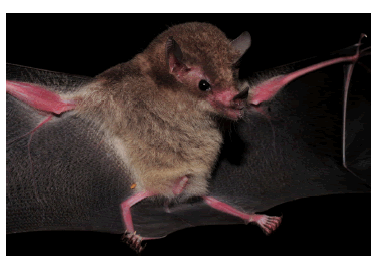
\includegraphics{../RMarkdown/bokermanni.png}
\caption{aaa}
\end{figure}

\begin{figure}

{\centering 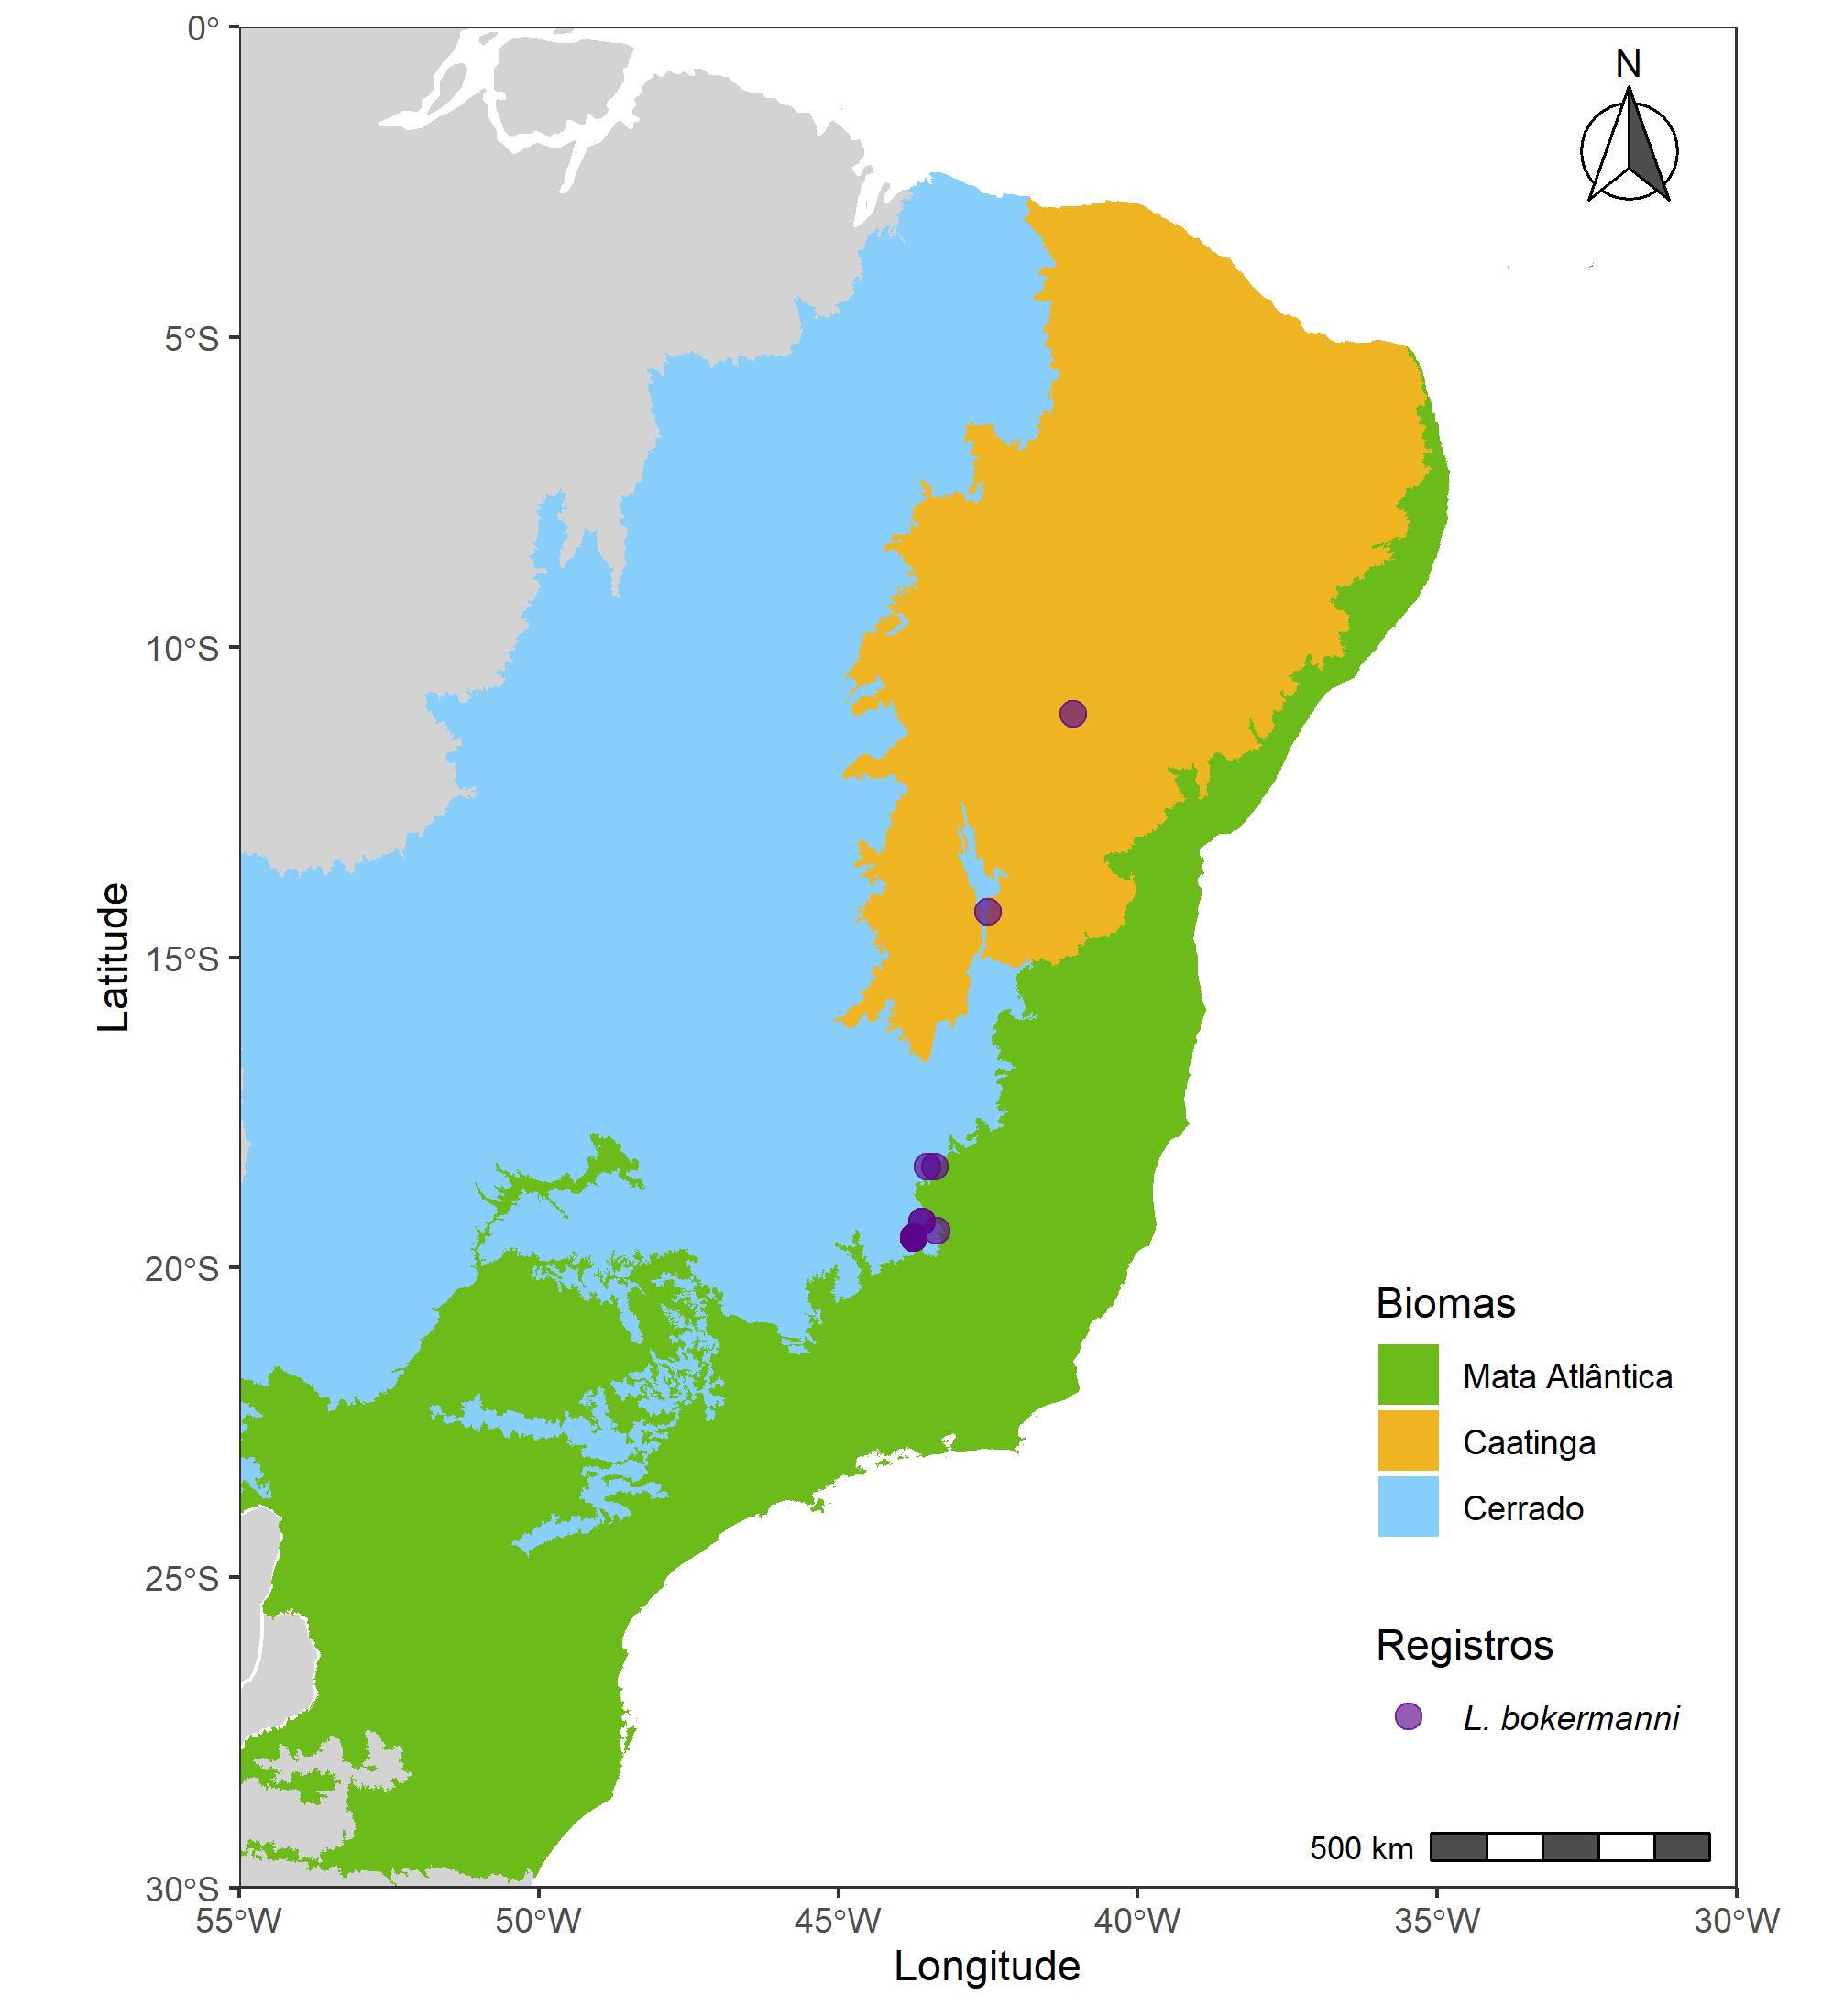
\includegraphics[width=0.49\linewidth]{../Graficos/Figure_1} 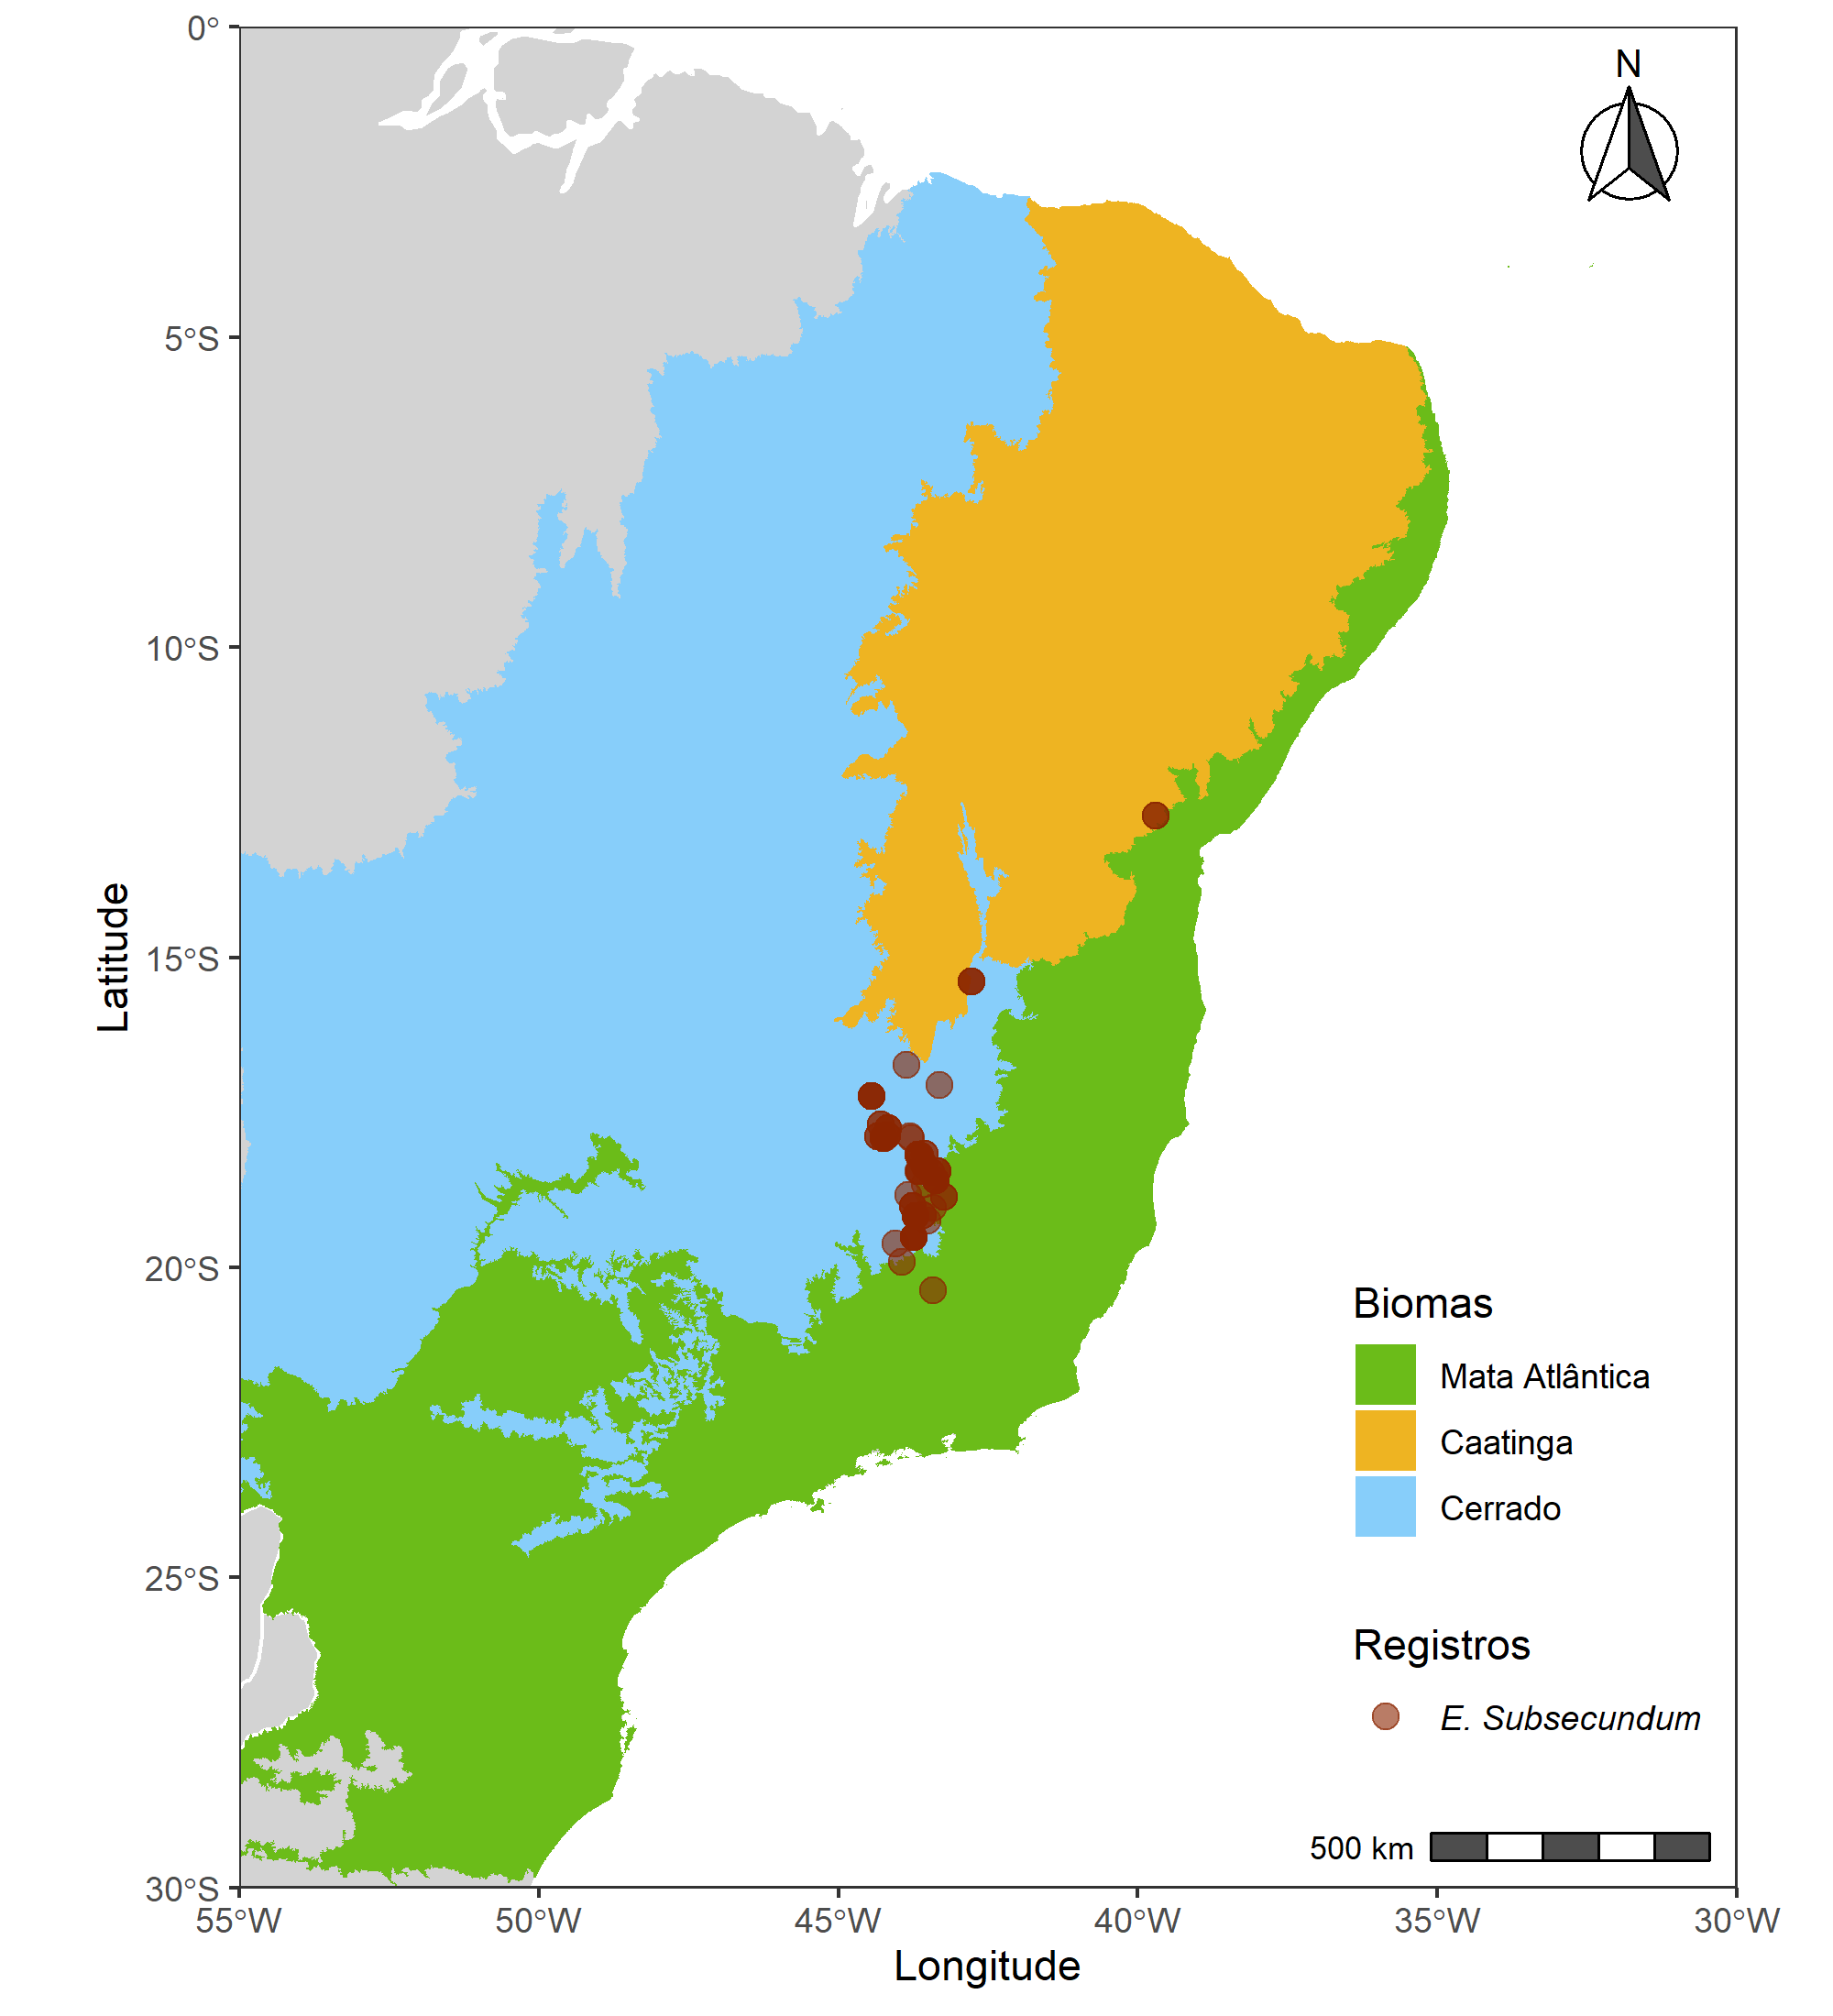
\includegraphics[width=0.49\linewidth]{../Graficos/Figure_2} 

}

\caption{Gráfico das localidades de L. bokermanni (à esquerda) e E. subsecundum (à direita)}\label{fig:plot_bokermanni}
\end{figure}

\hypertarget{modelo-de-distribuiuxe7uxe3o}{%
\subsection{Modelo de Distribuição}\label{modelo-de-distribuiuxe7uxe3o}}

\hypertarget{dados-ambientais}{%
\subsection{Dados ambientais}\label{dados-ambientais}}

~~~~Para produzir os modelos de distribuição potencial das espécies
utilizamos camadas ambientais obtidas do projeto WorldClim
{[}@worldclim{]}, com resolução espacial de 2.5 arc-minutos
(aproximadamente 4.5 km no equador) e representando o clima atual,
correspondendo à média das observações de 1970 a 2000. As 19 variáveis
bioclimáticas \protect\hyperlink{apuxeandice}{Tabela 3} derivam de dados
de temperatura e precipitação, repesentando tendências anuais, condições
extremas e sazionalidade {[}@worldclim{]}.

Para as predições de distribuições futuras, utilizamos camadas
projetadas do clima global para o ano de 2050 (média de 2041 a 2060) de
acordo com o Quinto Relatório de Avaliação do Painel Intergovernamental
sobre Mudanças Climáticas (AR5) do Painel Intergovernamental sobre
Mudanças Climáticas {[}@IPCC{]}, obtidas também através do projeto
WorldClim {[}@worldclim{]}. São camadas de 19 biovariáveis
\protect\hyperlink{apuxeandice}{Tabela 3} projetadas para o futuro, com
resolução de 2.5 arc-minutos e usando o modelo de circulação ACCESS1,
representando dois cenários distintos de emissão de gases do efeito
estufa conforme o \emph{Representative Concentration Pathways} (RCPs), o
de RCP 45 (cenário no qual as emissões de \(CO_2\) começam a diminuir a
partir de 2045) e de RCP 85 (as emissões de gases continuam a crescer ao
longo do século 21) {[}@Vuuren2011{]}.

Diversos autores apontaram problemas de multicolinearidade de variáveis
climáticas em modelagens de distribuição {[}@braunisch2013;
@cardenas2014{]}, afetando diretamente os resultados e performance dos
modelos. A fim de avaliar a gravidade da colinearidade entre os pontos
de ocorrências das duas espécies e o conjunto de biovariáveis do clima
atual, medimos o Fator de Inflação da Variância (VIF) das camadas
ambientais. Para os dados de ocorrência da planta \emph{E. subsecundum},
o teste resultou em 13 (de 19) variáveis bioclimáticas com problemas de
colinearidade \protect\hyperlink{apuxeandice}{Tabela 4}. Enquanto que
para o morcego \emph{L. bokermanni}, 17 variáveis apresentaram alto grau
de colinearidade \protect\hyperlink{apuxeandice}{Tabela 5}. Valores de
VIF maiores que o limiar 10 já indicam problema de colinearidade.

\begin{figure}

{\centering 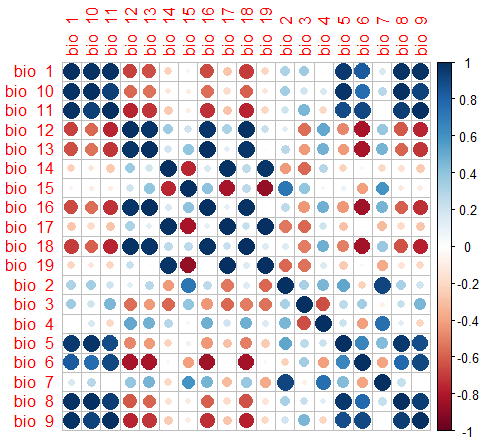
\includegraphics[width=0.49\linewidth]{../Dados/Resultados_VIF/E_subsecundum/Corr_plot_19_biovars} 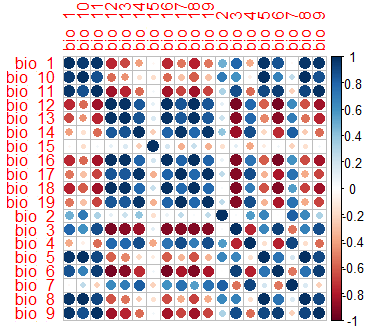
\includegraphics[width=0.49\linewidth]{../Dados/Resultados_VIF/L_bokermanni/Corr_plot_19_biovars} 

}

\caption{Matriz de correlação entre as variáveis bioclimáticas para a espécie E. subsecundum (à esquerda) e L. bokermanni (à direita)}\label{fig:VIF_subs}
\end{figure}

\end{document}
